% =====================================================================
%  TAORG / V-HPED -- IEEE conference paper (IEEEtran, conference mode)
%  All numbers come from saved run artifacts via make_artifacts.py
%  (provenance: supplementary/provenance.json).  All results are SYNTHETIC.
% =====================================================================
\documentclass[conference]{IEEEtran}
\IEEEoverridecommandlockouts

\usepackage{cite}
\usepackage{amsmath,amssymb,amsfonts}
\usepackage{graphicx}
\usepackage{booktabs}
\usepackage{algorithm}
\usepackage{algpseudocode}
\usepackage{xcolor}
\usepackage{url}
\usepackage{tikz}
\usetikzlibrary{arrows.meta,positioning,fit,calc}

\newtheorem{proposition}{Proposition}
\newtheorem{lemma}{Lemma}
\newtheorem{theorem}{Theorem}
\newcommand{\softplus}{\operatorname{softplus}}
\newcommand{\VIS}{\textsc{vis}}
\newcommand{\OCC}{\textsc{occ}}
\newcommand{\UNK}{\textsc{unk}}

\begin{document}

\title{Occluded or Ended? Visibility-Thinned Hawkes Filtering with Exact Lazy Maintenance for Video Scene-Graph Relationships}

\author{\IEEEauthorblockN{\textcolor{red}{[Author Name 1]}}
\IEEEauthorblockA{\textcolor{red}{[Department, Institution]}\\
\textcolor{red}{[City, Country]}\\
\textcolor{red}{[email]}}
\and
\IEEEauthorblockN{\textcolor{red}{[Author Name 2]}}
\IEEEauthorblockA{\textcolor{red}{[Department, Institution]}\\
\textcolor{red}{[City, Country]}\\
\textcolor{red}{[email]}}}

\maketitle

\begin{abstract}
Video scene-graph generators predict subject--predicate--object relationships frame by
frame, so a relationship that is briefly occluded or missed flickers, while temporal
smoothing keeps relationships alive after they have ended because it cannot tell
\emph{why} an edge stopped being observed. We present V-HPED, a model-agnostic
post-processing filter that treats the detections of a live relationship as a
self-exciting (Hawkes) point process thinned by a visibility-dependent detection
probability, and filters a latent alive/dead state with an exact, differentiable
forward likelihood. Under this observation model, a visible miss carries evidence
against the relationship proportional to its current intensity, whereas an occluded
miss is (nearly) censored. We also prove that, under two stated conditions, untouched
relationships evolve in closed form, which yields an exact lazy implementation with a
per-pair wake-up heap, and we show that the conditions cannot be dropped in general.
All experiments are synthetic; no real-video result is reported. On 5 predeclared
seeds with occlusion and detector flicker, fitted V-HPED drops terminated relationships
1.63~frames earlier than visibility-gated EMA (paired 95\% CI $[-1.87,-1.38]$) with
slightly higher frame-level F1 ($+0.008$, CI $[0.006,0.010]$) and lower calibration
error (ECE $0.030$ vs.\ $0.286$), but a visibility-only variant without Hawkes terms
attains the highest F1. Under synthetic identity switches, fitted V-HPED loses to
simpler baselines; we trace this to a confounding of identity-induced and
visibility-induced absence and report that a first identity-aware extension did not
fix it. Lazy maintenance matched the eager reference in every tested decision and was
up to $4.46\times$ faster when 5\% of pairs are updated per frame, but $0.77\times$ as
fast when all are.
\end{abstract}

\begin{IEEEkeywords}
video scene graphs, temporal point processes, Hawkes processes, occlusion, hidden
Markov filtering, calibration, lazy evaluation, priority queues
\end{IEEEkeywords}

% ---------------------------------------------------------------------
\section{Introduction}
% ---------------------------------------------------------------------
Video scene-graph generation (VidSGG) models such as STTran~\cite{cong2021sttran},
DSG-DETR~\cite{feng2023dsgdetr} and TEMPURA~\cite{nag2023tempura} output, at every
frame, a set of relationship triplets between tracked objects, typically evaluated on
Action Genome~\cite{ji2020ag}. Applications that consume these graphs need
relationship \emph{state}: is the person still holding the cup? Occlusion, missed
detections and tracker failures~\cite{zhang2022bytetrack} make continuing
relationships vanish for a few frames, which produces churn in frame-wise outputs.

A temporal memory bridges such gaps but faces a trade-off: slow decay persists through
occlusion and also through genuine termination; fast decay does the opposite. The
missing ingredient is the \emph{reason} for absence. If an object is occluded, the
absence of a detection is censored evidence; if both objects are clearly visible and
the relationship is not detected, absence is evidence that it ended---and its strength
should depend on how reliably the relationship has been detected so far.

We study this question with a post-hoc, model-agnostic layer and report, alongside the
positive findings, where it fails. Our contributions are:
\begin{enumerate}
\item \textbf{A visibility-thinned self-exciting observation model for edge
persistence (V-HPED).} We instantiate a Markov-modulated Hawkes
process~\cite{hawkes1971,wang2012mmhp} with visibility-dependent
thinning~\cite{lewis1979} and an exact forward filter~\cite{rabiner1989} over a latent
alive/dead state per relationship, including a cross-predicate termination hazard. We
derive its censoring, evidence-strength and nesting properties
(Props.~\ref{prop:censor}--\ref{prop:nest}). The components are established; the
contribution is their formulation for VidSGG edge persistence and its evaluation.
\item \textbf{Exact lazy maintenance.} We prove that two conditions make untouched
relationships evolve in closed form (Lemma~\ref{lem:semigroup}), give a per-pair
wake-up heap that preserves the eager filter's outputs (Theorem~\ref{thm:equiv}),
show that the conditions are necessary in the generic case
(Prop.~\ref{prop:necessity}), and measure where the optimisation helps and hurts.
\item \textbf{A controlled synthetic study with failure analysis.} Using paired
corruption manifests, five predeclared seeds and validation-only threshold
selection, we compare V-HPED with five baselines and five ablations, diagnose its
failure under identity switches as a confounding of identity- and
visibility-induced absence, report a negative result for a first identity-aware
extension, and document limits of parameter identifiability.
\end{enumerate}

% ---------------------------------------------------------------------
\section{Related Work}
% ---------------------------------------------------------------------
\textbf{Video scene graphs.} Action Genome~\cite{ji2020ag} annotates person--object
relationships on sampled frames. STTran~\cite{cong2021sttran}, DSG-DETR~\cite{feng2023dsgdetr}
and TEMPURA~\cite{nag2023tempura} model temporal context inside the network; TEMPURA
additionally attenuates label noise with uncertainty modelling. RTAformer~\cite{heo2026rtaformer}
targets the opposite failure---keeping a stale predicate after a relation changes---by
separating entity persistence from relation change. World scene-graph
generation~\cite{peddi2026wsgg} keeps unobserved objects in a persistent 3-D world
frame and annotates their relationships; TCDSG~\cite{ruschel2024tcdsg} enforces
identity consistency end to end. From their abstracts, none of these outputs a
calibrated probability that a relationship has ended or separates censored from
negative evidence; V-HPED is a post-hoc layer and is complementary rather than a
competitor to these networks. We did not compare against them empirically.

\textbf{Temporal point processes.} Hawkes processes~\cite{hawkes1971} and neural
variants~\cite{mei2017} model self-exciting event streams, including dynamic knowledge
graphs~\cite{trivedi2017}. Markov-modulated Hawkes processes~\cite{wang2012mmhp} let a
hidden state switch the excitation dynamics, which is the mathematical family V-HPED
belongs to. Thinning~\cite{lewis1979} and detection functions for missing Hawkes
events~\cite{deutsch2020} are established. Dynamic occupancy
models~\cite{mackenzie2003} combine a latent presence state, colonisation/extinction
and imperfect, covariate-dependent detection---a close ecological analogue of
relationship persistence under occlusion.

\textbf{Tracking and identity.} Multi-object trackers such as
ByteTrack~\cite{zhang2022bytetrack} produce the identities on which relationships are
keyed. Labeled random-finite-set filters delay track termination when occlusion is
likely~\cite{kim2016lrfs}, and probabilistic data association weights evidence by its
association probability~\cite{barshalom1975}; both concern object tracks rather than
relationship edges.

\textbf{Calibration.} We report expected calibration error~\cite{guo2017calibration}
of the alive probability, which matters when downstream modules threshold or fuse it.

% ---------------------------------------------------------------------
\section{Problem Formulation}
% ---------------------------------------------------------------------
A base VidSGG model and tracker emit, for every frame $n$ with timestamp $t_n$
($\Delta_n=t_n-t_{n-1}$; the first interval is $1/\mathrm{fps}$), records for
subject--object pairs $k=(i,j)$ of track labels and predicates $p\in\{1,\dots,P\}$:
an indicator $o^p_{k,n}\in\{0,1\}$ (predicted or not), a score $w^p_{k,n}\in[0,1]$ and
the visibility of both tracks. A pair's regime $v_{k,n}\in\{\VIS,\OCC,\UNK\}$ is the
most conservative of its records (\OCC{} dominates \UNK{}, which dominates \VIS{}); a
pair with no record in a frame is \UNK, never silently \VIS. After a predicate is first
observed on a pair, later frames that list the pair carry explicit absence records.
The task is to output, causally at each frame, the set of edges $(k,p)$ whose
relationship is still ongoing, together with a score.

% ---------------------------------------------------------------------
\section{Proposed Method: V-HPED}
% ---------------------------------------------------------------------
Fig.~\ref{fig:arch} shows the data flow. V-HPED keeps, per active pair, excitation
traces $\mathbf e_k\in\mathbb R^P_{\ge0}$ and per tracked predicate a belief
$a^p_k=P(A^p_k=1\mid o_{\le n})$ that the relationship is alive.

\begin{figure}[t]
\centering
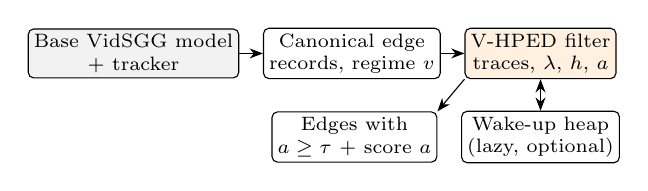
\begin{tikzpicture}[font=\scriptsize, node distance=3mm,
  box/.style={draw, rounded corners=2pt, align=center, minimum height=6mm, inner sep=2pt},
  >=Stealth]
\node[box, fill=gray!10] (base) {Base VidSGG model\\+ tracker};
\node[box, right=of base] (stream) {Canonical edge\\records, regime $v$};
\node[box, right=of stream, fill=orange!12] (filt) {V-HPED filter\\traces, $\lambda$, $h$, $a$};
\node[box, below=4mm of filt] (heap) {Wake-up heap\\(lazy, optional)};
\node[box, left=of heap] (out) {Edges with\\ $a\ge\tau$ + score $a$};
\draw[->] (base) -- (stream);
\draw[->] (stream) -- (filt);
\draw[<->] (filt) -- (heap);
\draw[->] (filt.south west) -- (out.north east);
\end{tikzpicture}
\caption{Data flow. The temporal layer consumes canonical per-frame records and emits
the edges whose alive probability passes a threshold selected on validation data.}
\label{fig:arch}
\end{figure}

\subsection{Self-exciting intensity and hazard}
Before the frame-$n$ update the traces decay with a regime-dependent rate,
\begin{equation}
e_q \leftarrow e_q\, e^{-\beta_{v_n}\Delta_n},\qquad \beta_{\VIS},\beta_{\OCC},\beta_{\UNK}>0,
\label{eq:decay}
\end{equation}
and after it they add the frame's marks, $e_q\leftarrow e_q+o^q_n w^q_n$. The
detection intensity and termination hazard (both in s$^{-1}$) are
\begin{align}
\lambda_p &= \softplus\!\Big(\mu_p+\textstyle\sum_q \alpha_{qp}e_q\Big),\label{eq:lambda}\\
h_p &= \softplus\!\Big(\eta_p+\textstyle\sum_q \gamma_{qp}e_q\Big).\label{eq:hazard}
\end{align}
The softplus keeps both positive for any sign of $\alpha,\gamma$ (inhibition is valid).
$\gamma_{qp}$ lets predicate $q$ raise or lower the hazard that $p$ ends.
($\texttt{temporal/vhped/dynamics.py}$.)

\subsection{Visibility-thinned observation model}
Absence is \emph{not} modelled as a Hawkes event. If the relationship is alive,
detections arrive with intensity $\rho_v\lambda_p$; if it is dead, spurious detections
arrive with rate $\rho_v\varepsilon$, where $\rho_{\VIS}=1$ and
$\rho_{\OCC},\rho_{\UNK}\in[0,1]$ are thinning probabilities. With the intensity held
at its left limit over a frame,
\begin{equation}
L_1\!=\!P(o\!=\!1\mid A\!=\!1)=1-e^{-\rho_v\lambda_p\Delta},\;\;
L_0\!=\!P(o\!=\!1\mid A\!=\!0)=1-e^{-\rho_v\varepsilon\Delta}.
\label{eq:emission}
\end{equation}
Because the model is defined on frames, the compensator is exactly
$\rho_v\lambda_p\Delta$; no integral of the softplus intensity is needed. Relative to a
continuous-time process this is a left-Riemann approximation (an assumption).

\subsection{Alive/dead filter and likelihood}
The latent state follows a two-state continuous-time Markov chain with rates $h_p$
(alive$\to$dead) and $r$ (dead$\to$alive), giving the exact transition
\begin{equation}
a^- = \pi + (a-\pi)\,e^{-(h_p+r)\Delta},\qquad \pi=r/(h_p+r),
\label{eq:predict}
\end{equation}
followed by the Bayes update with the record's likelihoods
$\ell_1=L_1^{o}(1-L_1)^{1-o}$, $\ell_0=L_0^{o}(1-L_0)^{1-o}$:
\begin{equation}
c=a^-\ell_1+(1-a^-)\ell_0,\qquad a = a^-\ell_1/c.
\label{eq:update}
\end{equation}
A predicate becomes tracked at its first detection with prior $a=\pi_0$ and then
receives the same predict/update step. The log-likelihood
$\sum_n\sum_{(k,p)\text{ tracked}}\log c$ is exact for this discrete model and is
implemented twice: in NumPy for inference and in PyTorch for fitting
($\texttt{alive.py}$, $\texttt{likelihood.py}$); a test asserts agreement to
$10^{-9}$. Parameters are fitted by maximum likelihood on training videos only
(Adam, 200 iterations, learning rate 0.05, $L_2$ penalty $10^{-3}$ on off-diagonal
$\alpha$ and on $\gamma$; positivity by softplus, probabilities by sigmoid). The
keep/drop threshold $\tau$ on $a$ is selected on validation videos. Predicates whose
belief falls below $10^{-6}$ are pruned.

\begin{proposition}[Censoring]\label{prop:censor}
If $\rho_v=0$, an absence leaves the belief unchanged except for the prior transition
\eqref{eq:predict}.
\end{proposition}
\begin{proposition}[Evidence of a visible miss]\label{prop:evidence}
For $\rho_v=1$ and $o=0$,
$\log\big[(1-L_1)/(1-L_0)\big]=-(\lambda_p-\varepsilon)\Delta$.
\end{proposition}
Both follow by substitution into \eqref{eq:emission}. Prop.~\ref{prop:evidence} is the
behavioural difference from visibility-gated EMA: the evidence that a relationship
ended grows with its current intensity, i.e.\ with how densely and recently it was
detected.
\begin{proposition}[Nesting]\label{prop:nest}
With $\alpha=\gamma=0$ and $\rho\equiv1$, V-HPED equals a two-state HMM with constant
emissions; this is checked numerically against our HMM baseline (agreement to $10^{-10}$).
\end{proposition}
This yields the ablation ladder HMM $\subset$ VT-HMM ($+$visibility, $\alpha=\gamma=0$)
$\subset$ V-HPED self-only $\subset$ V-HPED.

% ---------------------------------------------------------------------
\section{Exact Lazy Maintenance}
% ---------------------------------------------------------------------
The eager reference updates every active pair every frame. Call a pair
\emph{touched} in a frame if it has at least one record.

\begin{lemma}[Untouched semigroup]\label{lem:semigroup}
Assume (L1) $\rho_{\UNK}=0$ and (L2) $\gamma=0$. For an untouched pair, one eager step
over $\Delta$ maps $e\mapsto e\,e^{-\beta_{\UNK}\Delta}$ and
$a^p\mapsto\pi_p+(a^p-\pi_p)e^{-(h_p+r)\Delta}$ with constant
$h_p=\softplus(\eta_p)$, and adds zero log-likelihood. Hence after untouched frames
from $t_0$ to $t$ the state depends only on $t-t_0$.
\end{lemma}
\emph{Proof.} With $\rho=0$ and $o=0$, $\ell_1=\ell_0=1$, so \eqref{eq:update} returns
$a^-$ and $c=1$; by (L2) the hazard does not depend on the traces; both maps form
semigroups in $\Delta$. \hfill$\square$

Under Lemma~\ref{lem:semigroup} each belief is monotone in time, so it crosses the
threshold $\tau$ or the prune level at most once, at a closed-form delay
$d^\ast=\ln\!\big[(a_0-\pi)/(L-\pi)\big]/(h+r)$ when $a_0$ and $\pi$ lie on opposite
sides of the level $L$ (otherwise never). Each pair keeps one authoritative
\emph{wake-up}: the earliest such crossing. Wake-ups may be early (the pair was touched
since), which is safe because popping only re-evaluates the closed form; superseded
heap entries are skipped by a wake id. Algorithm~\ref{alg:lazy} lists one frame
($\texttt{temporal/vhped/lazy.py}$, $\texttt{expiry\_heap.py}$).

\begin{algorithm}[t]
\caption{Lazy V-HPED frame step (exact under L1, L2)}
\label{alg:lazy}
\begin{algorithmic}[1]
\For{each touched pair $k$ (incl.\ new pairs with a detection)}
  \State materialise $k$ to $t_{n-1}$ with Lemma~\ref{lem:semigroup}
  \State run the eager step \eqref{eq:decay}--\eqref{eq:update}; update output set
  \State $w\gets t_n+\min_p d^\ast_p$ \Comment{threshold and prune levels}
  \If{no pending wake-up $\le w$} push $(w,k,\text{new id})$ \EndIf
\EndFor
\While{heap minimum $<t_n$}
  \State pop; skip if its id is stale
  \State re-evaluate $k$ at $t_n$ by Lemma~\ref{lem:semigroup}; apply crossings and prunes
  \State push the next wake-up of $k$ (if finite)
\EndWhile
\State emit the output set with scores evaluated at $t_n$
\end{algorithmic}
\end{algorithm}

\begin{theorem}[Equivalence]\label{thm:equiv}
Under (L1)--(L2) and exact arithmetic, Algorithm~\ref{alg:lazy} emits the same edges,
scores and log-likelihood as the eager filter at every frame.
\end{theorem}
\emph{Proof sketch.} Touched pairs are materialised by Lemma~\ref{lem:semigroup} and then
receive the identical eager step. An untouched pair's membership changes only at a
crossing; the pending wake-up is never later than the earliest true crossing (pushes
keep the minimum, pops recompute from the exact state), and crossings are applied at
the first frame whose time exceeds them, matching the eager comparison $a\ge\tau$.
Untouched frames add zero log-likelihood. \hfill$\square$

In floating point the eager filter composes per-frame exponentials and the lazy one a
single exponential; we therefore test scores to relative $10^{-9}$ and allow decision
differences only within $10^{-9}$ of $\tau$.

\begin{proposition}[Necessity, generic case]\label{prop:necessity}
If $\rho_{\UNK}>0$ or $\gamma_{\cdot p}\neq0$, and $e\neq0$, $\lambda\neq\varepsilon$,
$h>0$, the eager belief after elapsed time $D$ depends on how $D$ is split into frames;
hence no function of $(\text{state},D)$ reproduces it.
\end{proposition}
\emph{Reason.} Each untouched frame multiplies the odds by
$e^{-\rho_{\UNK}(\lambda(t_n)-\varepsilon)\Delta_n}$ (or the survival by
$e^{-h(t_n)\Delta_n}$) with a trace-dependent, decaying rate, i.e.\ a partition-dependent
Riemann sum interleaved with a non-commuting predict step. We verified this numerically:
four partitions of $0.3$\,s give beliefs differing by more than $10^{-4}$ when a condition
is violated and agreeing to $10^{-12}$ when both hold. This is a statement about this
discrete-time filter, not a general theorem.

\textbf{Complexity.} Per frame, eager maintenance costs $\Theta(AP)$ for $A$ active pairs.
Lazy maintenance costs $O(k_{\mathrm{t}}P+(k_{\mathrm{t}}+k_{\mathrm{w}})(P+\log H))$ for
$k_{\mathrm{t}}$ touched pairs, $k_{\mathrm{w}}$ valid wake-ups and heap size $H$, with at
most one push per touch or wake-up; a stale-entry scan runs only after the heap doubles,
keeping $H=O(A)$ amortised (argued, not separately tested). Emitting the output set costs
$O(|S|)$ in both and is counted separately. Lazy is faster only if
$k_{\mathrm t}/A$ is below roughly $c_E/(c_L+c_W)$, the ratio of per-step costs; when
every pair is touched there is nothing to skip.

% ---------------------------------------------------------------------
\section{Identity Switches and an Identity-Aware Extension}
% ---------------------------------------------------------------------
Records are keyed by track labels, so an identity switch between objects $A$ and $B$
moves a relationship from the real pair to a \emph{phantom} pair and back. In our
encoding the real pair has no records during the swap (\UNK) while still alive, and
after the swap the phantom pair has no records while never having existed. One global
$\rho_{\UNK}$ must explain both (Sec.~\ref{sec:results-id} measures the consequence).

As a first remedy (IA-v1, $\texttt{temporal/vhped\_ia/}$) we let a tracker score
$\kappa_{i,n}\in[0,1]$ define a per-track belief
$\zeta_i\leftarrow\kappa\zeta_i+(1-\kappa)(1-\zeta_i)$ that label $i$ still refers to its
original object (two-object swap model), and mix, per pair with
$\zeta_k=\zeta_i\zeta_j$,
\begin{equation}
P(o\mid\cdot)=\zeta_k\prod_p c_p+(1-\zeta_k)\prod_p Q(o_p),\;\;
a_p=w\,a_p^{\mathrm{post}}+(1-w)\,\bar a_p,
\label{eq:ia}
\end{equation}
where $Q(o{=}1)=1-e^{-\rho_v\phi\Delta}$ is a state-independent foreign-detection
model, $w$ is the posterior that the pair is identity-consistent, and $\bar a_p$ is the
prediction (or a learned belief $b$ for predicates first seen on an inconsistent pair).
With $\kappa\equiv1$ it reduces exactly to V-HPED (tested); Lemma~\ref{lem:semigroup}
still applies because untouched pairs have unit likelihood factors. IA-v1 reads $\kappa$
as a calibrated non-jump probability; Sec.~\ref{sec:results-id} shows this assumption
failed. A calibrated variant, $P(\text{jump}\mid\kappa)=\sigma(a+b\,\mathrm{logit}(1-\kappa))$
with $(a,b)$ learned (IA-v2), is implemented and unit-tested but \emph{has not been
evaluated}.

% ---------------------------------------------------------------------
\section{Experimental Setup}
% ---------------------------------------------------------------------
\textbf{Data (synthetic only).} Each video has 150 frames at 30\,fps and four
subject--object pairs with three predicates: \emph{holding} (ends while both objects are
visible with probability 0.6, at a frame in $[40,120]$), a 6-frame \emph{putting-down}
cue before \emph{holding} ends, and an independent \emph{looking-at}. Each edge has a
detector reliability drawn from $\{0.95,0.75,0.5\}$; dead edges produce spurious
detections with probability 0.02 per frame; scores are $U(0.5,1)$. Two pair-level
occlusion gaps of $\{3,5,10,20\}$ frames per pair suppress detections and set the
regime to \OCC; they are recorded in deterministic corruption manifests.
\emph{Condition A}: occlusion + flicker. \emph{Condition B}: A plus two same-class
identity swaps of 5 frames per video. Further conditions (Table~\ref{tab:ia}) vary
the number of swaps, add visibility-label flips (10\%) or timestamp jitter ($\pm50\%$),
and attach a simulated identity score whose informativeness $s\in[0,1]$ is controlled
(normal frames $\kappa\sim U(0.9,1)$; swap frames shifted down by $0.85s$; 1\% false
alarms).

\textbf{Protocol.} Per seed (5 predeclared seeds: 42, 123, 456, 789, 2024): 20 training,
10 validation and 20 test videos. Fitted variants use training streams only; every
method's threshold is chosen on validation by frame-level F1 from a 20-point grid; test
results are reported at that threshold as mean$\pm$std over seeds. All methods see
identical corrupted streams. Paired differences use a percentile bootstrap (10\,000
resamples) over the 100 test videos (99 with a terminating edge for delay).

\textbf{Baselines and ablations.} No memory; fixed window ($w{=}5$); EMA
($\alpha{=}0.3$, decay 0.9); visibility-gated EMA (decay 0.7 when visible, 0.95 when
occluded); hand-set two-state HMM; hand-set V-HPED; fitted VT-HMM ($\alpha{=}\gamma{=}0$),
V-HPED without visibility ($\rho\equiv1$), self-only ($\alpha,\gamma$ diagonal), full, and
a lazy-exact variant ($\gamma{=}0$, $\rho_{\UNK}{=}0$) run with Algorithm~\ref{alg:lazy}.

\textbf{Metrics} (definitions frozen before use; $\texttt{research/metric\_definitions.md}$).
F1$_{\mathrm{fr}}$: frame-level edge F1 against the uncorrupted ground truth (used for
threshold selection). F1$_{\mathrm{pers}}$: F1 inside injected occlusion intervals.
Delay: frames from the last ground-truth frame of a terminating edge to the first frame
it is dropped (censored at the video end). FPR: fraction of post-termination frames in
which the edge is still output. Churn: output state flips per consecutive frame pair
within an edge's ground-truth window. ECE (10 bins) and Brier score of the output score
on every tracked edge-frame. Latency: wall-clock ms per frame of the temporal layer
(Python, one Windows machine).

\textbf{Implementation checks.} The repository's test suite (282 tests at the time of
writing) covers the propositions, NumPy/PyTorch likelihood agreement, the HMM nesting,
eager--lazy equivalence on 24 randomized streams, and agreement between a vectorised
threshold sweep and the reference metric code. These checks support implementation
correctness only, not predictive performance.

% ---------------------------------------------------------------------
\section{Results and Discussion}
% ---------------------------------------------------------------------
\subsection{Occlusion and detector flicker (condition A)}
Table~\ref{tab:condA} and Fig.~\ref{fig:tradeoff} summarise condition A.
Fitted V-HPED has the highest persistence F1 (shared with VT-HMM), a termination delay of
3.37 frames versus 5.05 for visibility-gated EMA (paired difference $-1.63$, CI
$[-1.87,-1.38]$), lower false persistence (0.077 vs.\ 0.105) and a small frame-F1 gain
($+0.008$, CI $[0.006,0.010]$; Table~\ref{tab:paired}). Its alive probability is far
better calibrated (ECE 0.030 vs.\ 0.286; Brier 0.045 vs.\ 0.174), although EMA scores
are not designed as probabilities. Removing visibility collapses persistence through
occlusion (F1$_{\mathrm{pers}}$ 0.571). However, VT-HMM---visibility without Hawkes
terms---attains the best frame F1 (0.969 vs.\ 0.958; difference $-0.011$, CI
$[-0.013,-0.009]$), while terminating more slowly (5.26 frames). The Hawkes terms
therefore buy faster termination and calibration, not uniformly higher accuracy. The
cross-predicate terms add little over self-only (F1 $+0.003$). The lazy-exact variant
loses 0.001 F1 and 0.24 frames of delay relative to the full model.

\begin{table}[t]
\caption{Condition A (synthetic): occlusion + detector flicker. Test mean $\pm$ std over
5 seeds at the validation-selected threshold. No memory has trivially the shortest
delay because it never persists. Run \texttt{20261027\_202753\_a7314fe5}.}
\label{tab:condA}
\centering\scriptsize
\resizebox{\columnwidth}{!}{\begin{tabular}{@{}lcccccc@{}}
\toprule
Method & F1$_{\mathrm{fr}}\uparrow$ & F1$_{\mathrm{pers}}\uparrow$ & Delay$\downarrow$ & FPR$\downarrow$ & Churn$\downarrow$ & ECE$\downarrow$ \\
\midrule
No memory & 0.774\,$\pm$\,0.005 & 0.000\,$\pm$\,0.000 & \textbf{1.02\,$\pm$\,0.01} & \textbf{0.018\,$\pm$\,0.002} & 0.257\,$\pm$\,0.013 & 0.227\,$\pm$\,0.002 \\
Fixed window & 0.903\,$\pm$\,0.006 & 0.505\,$\pm$\,0.040 & 4.31\,$\pm$\,0.14 & 0.131\,$\pm$\,0.011 & \textbf{0.032\,$\pm$\,0.004} & 0.170\,$\pm$\,0.004 \\
EMA & 0.931\,$\pm$\,0.005 & 0.732\,$\pm$\,0.038 & 7.83\,$\pm$\,0.94 & 0.135\,$\pm$\,0.026 & 0.045\,$\pm$\,0.006 & 0.204\,$\pm$\,0.007 \\
Vis.-gated EMA & 0.950\,$\pm$\,0.002 & 0.922\,$\pm$\,0.012 & 5.05\,$\pm$\,0.61 & 0.105\,$\pm$\,0.025 & 0.040\,$\pm$\,0.015 & 0.286\,$\pm$\,0.004 \\
HMM (hand-set) & 0.890\,$\pm$\,0.007 & 0.269\,$\pm$\,0.027 & 2.37\,$\pm$\,0.08 & 0.041\,$\pm$\,0.003 & 0.088\,$\pm$\,0.008 & 0.206\,$\pm$\,0.005 \\
V-HPED hand-set & 0.950\,$\pm$\,0.004 & 0.921\,$\pm$\,0.020 & 4.17\,$\pm$\,0.38 & 0.072\,$\pm$\,0.009 & 0.036\,$\pm$\,0.005 & \textbf{0.013\,$\pm$\,0.002} \\
VT-HMM (fit) & \textbf{0.969\,$\pm$\,0.002} & 0.951\,$\pm$\,0.007 & 5.26\,$\pm$\,0.45 & 0.089\,$\pm$\,0.007 & 0.050\,$\pm$\,0.002 & 0.054\,$\pm$\,0.002 \\
V-HPED w/o vis. (fit) & 0.922\,$\pm$\,0.009 & 0.571\,$\pm$\,0.089 & 3.92\,$\pm$\,0.65 & 0.080\,$\pm$\,0.020 & 0.036\,$\pm$\,0.005 & 0.060\,$\pm$\,0.012 \\
V-HPED self-only (fit) & 0.955\,$\pm$\,0.006 & 0.946\,$\pm$\,0.011 & 3.53\,$\pm$\,0.40 & 0.074\,$\pm$\,0.012 & 0.041\,$\pm$\,0.007 & 0.033\,$\pm$\,0.012 \\
V-HPED (fit) & 0.958\,$\pm$\,0.007 & \textbf{0.951\,$\pm$\,0.011} & 3.37\,$\pm$\,0.30 & 0.077\,$\pm$\,0.015 & 0.038\,$\pm$\,0.008 & 0.030\,$\pm$\,0.014 \\
V-HPED lazy-exact (fit) & 0.956\,$\pm$\,0.008 & 0.948\,$\pm$\,0.012 & 3.63\,$\pm$\,0.43 & 0.075\,$\pm$\,0.012 & 0.039\,$\pm$\,0.008 & 0.030\,$\pm$\,0.015 \\
\bottomrule
\end{tabular}
}
\end{table}

\begin{table}[t]
\caption{Paired differences, fitted V-HPED minus each method (positive $\Delta$F1 and
negative $\Delta$Delay favour V-HPED). 95\% bootstrap CIs over test videos.}
\label{tab:paired}
\centering\scriptsize
\resizebox{\columnwidth}{!}{\begin{tabular}{@{}llcc@{}}
\toprule
Cond. & vs.\ method & $\Delta$F1$_{\mathrm{fr}}$ [95\% CI] & $\Delta$Delay [95\% CI] \\
\midrule
A & Vis.-gated EMA & +0.008 [+0.006, +0.010] & -1.63 [-1.87, -1.38] \\
A & V-HPED hand-set & +0.008 [+0.006, +0.010] & -0.73 [-0.94, -0.53] \\
A & VT-HMM (fit) & -0.011 [-0.013, -0.009] & -1.90 [-2.14, -1.67] \\
A & V-HPED w/o vis. (fit) & +0.037 [+0.032, +0.042] & -0.56 [-0.88, -0.24] \\
A & V-HPED self-only (fit) & +0.003 [+0.002, +0.004] & -0.15 [-0.22, -0.08] \\
B & Vis.-gated EMA & -0.015 [-0.018, -0.012] & -1.57 [-1.78, -1.36] \\
B & V-HPED hand-set & -0.033 [-0.036, -0.029] & -1.55 [-1.78, -1.33] \\
B & VT-HMM (fit) & -0.031 [-0.035, -0.028] & -0.83 [-0.99, -0.65] \\
B & V-HPED w/o vis. (fit) & +0.005 [-0.002, +0.012] & -1.57 [-1.87, -1.26] \\
B & V-HPED self-only (fit) & +0.003 [+0.002, +0.003] & -0.14 [-0.21, -0.08] \\
\bottomrule
\end{tabular}
}
\end{table}

\begin{figure}[t]
\centering
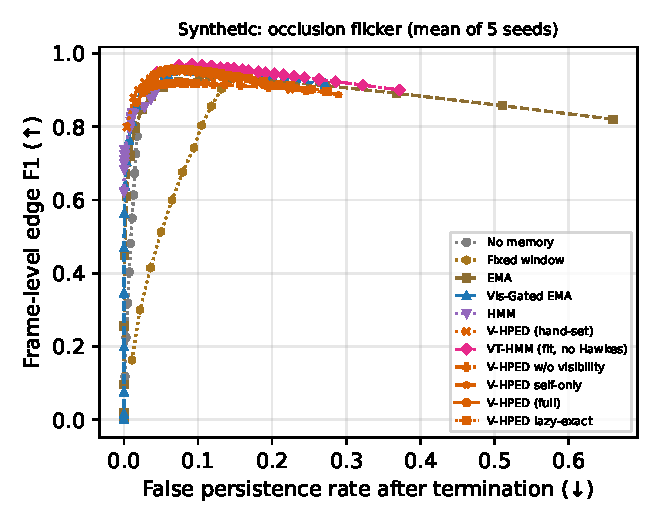
\includegraphics[width=0.49\columnwidth]{figures/tradeoff_occlusion_flicker.pdf}\hfill
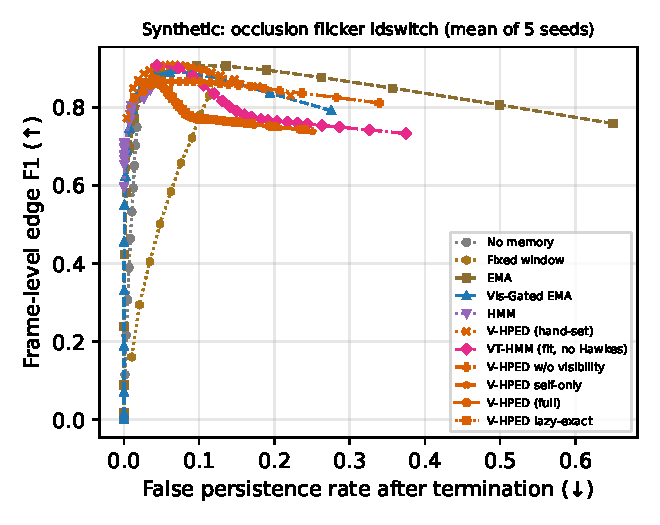
\includegraphics[width=0.49\columnwidth]{figures/tradeoff_occlusion_flicker_idswitch.pdf}
\caption{Frame F1 versus false persistence across thresholds (test, mean over seeds);
left: condition A, right: condition B. Synthetic.}
\label{fig:tradeoff}
\end{figure}

\subsection{Identity switches (condition B) and diagnosis}
\label{sec:results-id}
Under identity switches (Table~\ref{tab:condB}) fitted V-HPED still terminates fastest
among memory methods (2.12 frames) but loses frame F1 to visibility-gated EMA
($-0.015$, CI $[-0.018,-0.012]$, 0/5 seeds) and to its own hand-set version
(0.875 vs.\ 0.909), and its ECE rises to 0.211, with the threshold selected at the grid
edge (0.90) in all seeds. Two probes (Table~\ref{tab:probes}) test hypotheses about the
cause. Pinning the birth prior $\pi_0$ changes little (F1 0.882), falsifying an
over-confident-birth explanation. Pinning $\rho_{\UNK}$ during fitting recovers F1 0.919
and ECE 0.051: the fitted $\rho_{\UNK}$ had collapsed to $\approx0.006$ because the real
pair's identity-induced absence pushes it towards zero, which in turn censors the phantom
pair's absence forever. Pinning is a diagnostic, not a method.

IA-v1 did not fix the problem (Table~\ref{tab:ia}, Fig.~\ref{fig:dose}): it is worse than
fitted V-HPED in every switch condition (e.g.\ $-0.046$ F1 at 2 swaps), its results do not
depend on the informativeness $s$ of the identity score, and its fitted $\rho_{\UNK}$ still
collapses ($\approx0.004$). The cause is the calibration assumption: scores near
$U(0.9,1)$ on ordinary frames, read as non-jump probabilities, imply a $\approx5\%$ jump
chance per frame, so identity beliefs drift towards $1/2$ and all evidence is diluted.
Whether the learned calibration (IA-v2) resolves this is untested.

\begin{table}[t]
\caption{Condition B (synthetic): A plus two identity switches per video.}
\label{tab:condB}
\centering\scriptsize
\resizebox{\columnwidth}{!}{\begin{tabular}{@{}lcccccc@{}}
\toprule
Method & F1$_{\mathrm{fr}}\uparrow$ & F1$_{\mathrm{pers}}\uparrow$ & Delay$\downarrow$ & FPR$\downarrow$ & Churn$\downarrow$ & ECE$\downarrow$ \\
\midrule
No memory & 0.749\,$\pm$\,0.006 & 0.000\,$\pm$\,0.000 & \textbf{1.02\,$\pm$\,0.01} & \textbf{0.017\,$\pm$\,0.002} & 0.170\,$\pm$\,0.008 & 0.198\,$\pm$\,0.002 \\
Fixed window & 0.876\,$\pm$\,0.007 & 0.495\,$\pm$\,0.043 & 4.20\,$\pm$\,0.16 & 0.127\,$\pm$\,0.011 & \textbf{0.026\,$\pm$\,0.002} & 0.145\,$\pm$\,0.005 \\
EMA & 0.907\,$\pm$\,0.007 & 0.668\,$\pm$\,0.037 & 6.18\,$\pm$\,0.33 & 0.096\,$\pm$\,0.011 & 0.041\,$\pm$\,0.003 & 0.149\,$\pm$\,0.005 \\
Vis.-gated EMA & 0.891\,$\pm$\,0.005 & 0.878\,$\pm$\,0.015 & 3.74\,$\pm$\,0.22 & 0.061\,$\pm$\,0.003 & 0.050\,$\pm$\,0.005 & 0.192\,$\pm$\,0.005 \\
HMM (hand-set) & 0.861\,$\pm$\,0.007 & 0.258\,$\pm$\,0.030 & 2.29\,$\pm$\,0.10 & 0.039\,$\pm$\,0.003 & 0.063\,$\pm$\,0.005 & 0.172\,$\pm$\,0.004 \\
V-HPED hand-set & \textbf{0.909\,$\pm$\,0.005} & 0.876\,$\pm$\,0.029 & 3.74\,$\pm$\,0.46 & 0.060\,$\pm$\,0.011 & 0.029\,$\pm$\,0.004 & \textbf{0.028\,$\pm$\,0.003} \\
VT-HMM (fit) & 0.907\,$\pm$\,0.006 & 0.763\,$\pm$\,0.040 & 2.98\,$\pm$\,0.22 & 0.044\,$\pm$\,0.003 & 0.043\,$\pm$\,0.004 & 0.237\,$\pm$\,0.015 \\
V-HPED w/o vis. (fit) & 0.871\,$\pm$\,0.022 & 0.432\,$\pm$\,0.160 & 3.72\,$\pm$\,0.70 & 0.076\,$\pm$\,0.021 & 0.033\,$\pm$\,0.006 & 0.089\,$\pm$\,0.028 \\
V-HPED self-only (fit) & 0.873\,$\pm$\,0.008 & 0.877\,$\pm$\,0.019 & 2.29\,$\pm$\,0.27 & 0.039\,$\pm$\,0.005 & 0.060\,$\pm$\,0.007 & 0.210\,$\pm$\,0.014 \\
V-HPED (fit) & 0.875\,$\pm$\,0.007 & \textbf{0.895\,$\pm$\,0.016} & 2.12\,$\pm$\,0.24 & 0.038\,$\pm$\,0.004 & 0.059\,$\pm$\,0.007 & 0.211\,$\pm$\,0.013 \\
V-HPED lazy-exact (fit) & 0.871\,$\pm$\,0.010 & 0.859\,$\pm$\,0.060 & 2.21\,$\pm$\,0.19 & 0.038\,$\pm$\,0.003 & 0.062\,$\pm$\,0.008 & 0.215\,$\pm$\,0.014 \\
\bottomrule
\end{tabular}
}
\end{table}

\begin{table}[t]
\caption{Diagnostic probes in condition B (5 seeds; runs
\texttt{20261028\_044818\_696b2840}, \texttt{20261028\_045023\_e10fb99f}).
$\bar\tau$: mean selected threshold.}
\label{tab:probes}
\centering\scriptsize
\resizebox{\columnwidth}{!}{\begin{tabular}{@{}lcccc@{}}
\toprule
Method (cond.\ B) & F1$_{\mathrm{fr}}\uparrow$ & F1$_{\mathrm{pers}}\uparrow$ & ECE$\downarrow$ & $\bar\tau$ \\
\midrule
Vis.-gated EMA & 0.891\,$\pm$\,0.005 & 0.878\,$\pm$\,0.015 & 0.192\,$\pm$\,0.005 & 0.20 \\
V-HPED hand-set & 0.909\,$\pm$\,0.005 & 0.876\,$\pm$\,0.029 & 0.028\,$\pm$\,0.003 & 0.56 \\
V-HPED (fit) & 0.875\,$\pm$\,0.007 & 0.895\,$\pm$\,0.016 & 0.211\,$\pm$\,0.013 & 0.90 \\
V-HPED fit, $\pi_0{=}0.5$ pinned & 0.882\,$\pm$\,0.006 & 0.894\,$\pm$\,0.015 & 0.199\,$\pm$\,0.012 & 0.90 \\
V-HPED fit, $\rho_{\mathrm{unk}}{=}0.5$ pinned & 0.919\,$\pm$\,0.007 & 0.920\,$\pm$\,0.028 & 0.051\,$\pm$\,0.007 & 0.63 \\
V-HPED fit, $\rho_{\mathrm{unk}}{=}1$ pinned & 0.914\,$\pm$\,0.007 & 0.899\,$\pm$\,0.022 & 0.053\,$\pm$\,0.011 & 0.67 \\
\bottomrule
\end{tabular}
}
\end{table}

\begin{table}[t]
\caption{Frame-level F1 under further synthetic conditions (run
\texttt{20261028\_050001\_0c54b136}). $s$: informativeness of the simulated identity
score. The $\rho_{\mathrm{unk}}$-pinned column is a diagnostic.}
\label{tab:ia}
\centering\scriptsize
\resizebox{\columnwidth}{!}{\begin{tabular}{@{}lccccc@{}}
\toprule
Condition & Vis.-gated EMA & V-HPED hand-set & V-HPED (fit) & V-HPED fit, $\rho_{\mathrm{unk}}{=}0.5$ pinned & IA-v1 (fit) \\
\midrule
0 swaps & 0.950 & 0.950 & \textbf{0.958} & \textbf{0.958} & 0.955 \\
2 swaps, $s{=}1$ & 0.891 & 0.909 & 0.875 & \textbf{0.919} & 0.829 \\
2 swaps, $s{=}0$ & 0.891 & 0.909 & 0.875 & \textbf{0.919} & 0.829 \\
4 swaps, $s{=}1$ & 0.848 & 0.872 & 0.832 & \textbf{0.890} & 0.775 \\
2 sw., vis.\ flips & 0.884 & \textbf{0.894} & 0.837 & 0.888 & 0.812 \\
2 sw., jitter & 0.891 & 0.907 & 0.872 & \textbf{0.917} & 0.827 \\
\bottomrule
\end{tabular}
}
\end{table}

\begin{figure}[t]
\centering
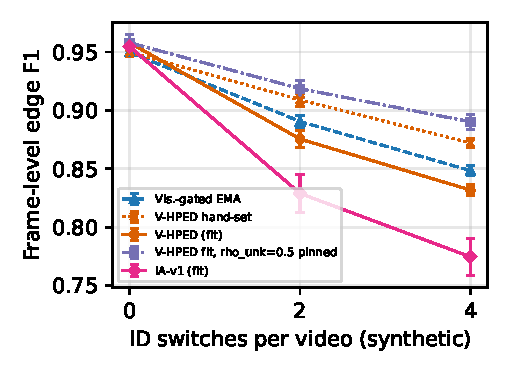
\includegraphics[width=0.8\columnwidth]{figures/idswitch_dose.pdf}
\caption{Frame F1 versus the number of identity switches per video (informative score,
$s{=}1$; mean $\pm$ std over 5 seeds). Synthetic.}
\label{fig:dose}
\end{figure}

\subsection{Efficiency of lazy maintenance}
Table~\ref{tab:eff} and Fig.~\ref{fig:eff} compare eager and lazy V-HPED on synthetic
traces with $A$ active pairs, $P=26$ predicates (two per pair) and a fraction $f$ of
pairs touched per frame (5 warm-up frames in which all pairs are touched, then 60
frames). Decision mismatches against the eager reference were zero at all 16 grid
points. At $A=3000$, lazy is $4.46\times$ faster at $f=0.05$ and $1.26\times$ at $f=0.5$,
but $0.77\times$ as fast at $f=1$, where nothing can be skipped and scheduling adds
about 30\% per update. Latency is machine-dependent; the update ratio is not. Memory
was not measured in this run.

\begin{table}[t]
\caption{Eager versus lazy per-frame update latency (ms) and work (one Windows machine,
Python; run \texttt{complexity/20261027T202322Z}).}
\label{tab:eff}
\centering\scriptsize
\resizebox{\columnwidth}{!}{\begin{tabular}{@{}rrrrrr@{}}
\toprule
$f$ & $A$ & Eager (ms) & Lazy (ms) & Speed-up & Lazy/eager updates \\
\midrule
0.05 & 300 & 10.08 & 1.86 & 5.41$\times$ & 0.128 \\
0.05 & 3000 & 110.87 & 24.87 & 4.46$\times$ & 0.125 \\
0.20 & 300 & 10.95 & 4.05 & 2.71$\times$ & 0.266 \\
0.20 & 3000 & 112.01 & 49.39 & 2.27$\times$ & 0.267 \\
0.50 & 300 & 10.63 & 8.17 & 1.30$\times$ & 0.546 \\
0.50 & 3000 & 114.58 & 91.22 & 1.26$\times$ & 0.546 \\
1.00 & 300 & 11.80 & 14.43 & 0.82$\times$ & 1.016 \\
1.00 & 3000 & 119.23 & 155.82 & 0.77$\times$ & 1.016 \\
\bottomrule
\end{tabular}
}
\end{table}

\begin{figure}[t]
\centering
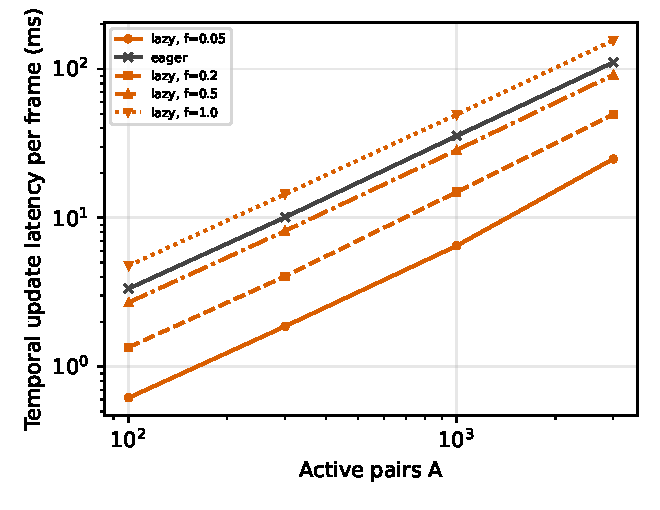
\includegraphics[width=0.49\columnwidth]{figures/complexity_latency.pdf}\hfill
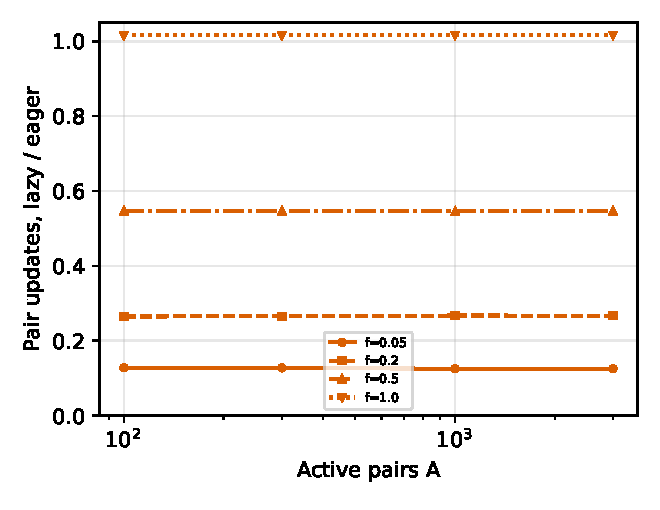
\includegraphics[width=0.49\columnwidth]{figures/complexity_work.pdf}
\caption{Latency (left) and the ratio of lazy to eager pair updates (right) versus the
number of active pairs, for touch fractions $f$.}
\label{fig:eff}
\end{figure}

\subsection{Parameter identifiability}
Simulating from known V-HPED parameters and refitting (5 seeds, 8 videos of 40 pairs,
Table~\ref{tab:recovery}) recovers the thinning $\rho_{\OCC}$ and spurious rate
$\varepsilon$ closely, but not $\mu$, $\alpha$ or $\beta$: the fitted values trade
baseline against excitation. Fitted intensity parameters should therefore be interpreted
only through behaviour. We have not established the cause of this trade-off; candidates
include the likelihood starting at each edge's first detection and weak separation of
$\mu$ and $\alpha$ near steady state.

\begin{table}[t]
\caption{Parameter recovery from data simulated by the model itself (run
\texttt{param\_recovery/20261028T051308Z}).}
\label{tab:recovery}
\centering\scriptsize
\begin{tabular}{@{}lccc@{}}
\toprule
Param. & True & Init. & Fitted (mean\,$\pm$\,std) \\
\midrule
$\mu$ & 3.00 & 5.00 & 13.56\,$\pm$\,0.36 \\
$\alpha_{pp}$ & 12.00 & 7.00 & 7.40\,$\pm$\,0.27 \\
$\eta$ & -1.00 & -0.50 & -0.29\,$\pm$\,0.07 \\
$\beta_{\mathrm{vis}}$ & 4.00 & 3.00 & 2.92\,$\pm$\,0.12 \\
$\beta_{\mathrm{occ}}$ & 0.50 & 0.30 & 0.24\,$\pm$\,0.05 \\
$\rho_{\mathrm{occ}}$ & 0.10 & 0.05 & 0.11\,$\pm$\,0.00 \\
$\varepsilon$ & 0.80 & 1.00 & 0.81\,$\pm$\,0.01 \\
\bottomrule
\end{tabular}

\end{table}

\subsection{Qualitative example}
Fig.~\ref{fig:qual} shows one synthetic relationship that is occluded and then ends.
V-HPED keeps it alive through the occlusion and drops it once the pair is visible again
without detections, whereas the visibility-gated EMA score decays steadily through the
occlusion. The dip near frame 90 illustrates a weakness: after dense detections, two
visible misses collapse the belief (Prop.~\ref{prop:evidence}), which contributes to churn.

\begin{figure}[t]
\centering
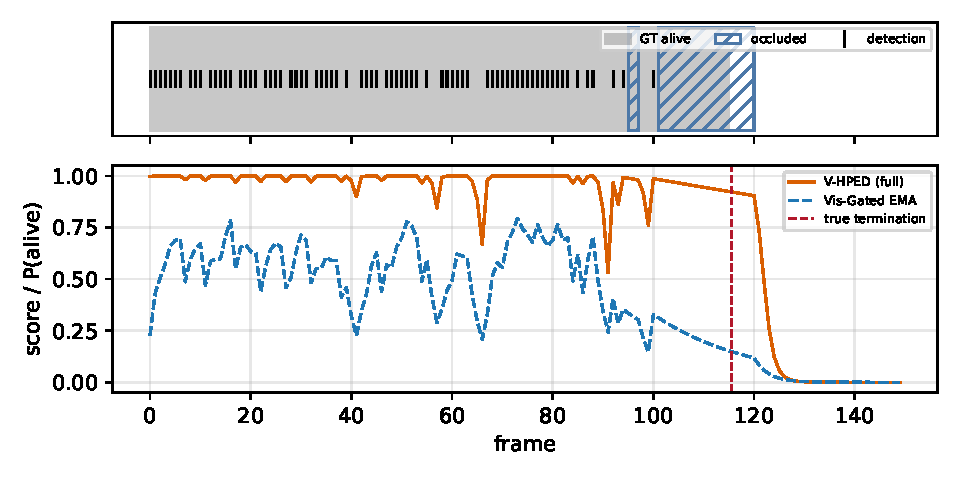
\includegraphics[width=\columnwidth]{figures/qualitative.pdf}
\caption{Illustrative synthetic sequence (not a statistic). Top: ground truth,
detections and occlusion. Bottom: fitted V-HPED alive probability and gated-EMA score.}
\label{fig:qual}
\end{figure}

% ---------------------------------------------------------------------
\section{Limitations and Threats to Validity}
% ---------------------------------------------------------------------
\begin{itemize}
\item \textbf{No real-data evidence.} All accuracy results are synthetic; the generator
uses the same visibility labels the methods consume and a simplified detector. An Action
Genome pilot and adapters for precomputed base-model predictions are implemented but have
not been run; claims about real detectors, trackers or base models are not made.
\item \textbf{Identity switches.} Fitted V-HPED is not robust to them in our encoding; the
identity-aware extension evaluated so far failed, and its calibrated variant is unevaluated.
\item \textbf{Accuracy versus termination.} A visibility-only HMM gives the highest frame F1
in condition A; the Hawkes terms help termination delay and calibration.
\item \textbf{Identifiability.} Intensity parameters are only weakly identified.
\item \textbf{Lazy exactness} requires $\rho_{\UNK}=0$ and $\gamma=0$; pairs touched under
occlusion are still updated eagerly, and lazy is slower when all pairs are touched.
\item \textbf{Novelty.} The model is an instance of Markov-modulated Hawkes processes with
thinning; the contribution is its formulation, analysis and evaluation for VidSGG edge
persistence. Our literature search was limited and abstract-level for recent preprints.
\item \textbf{Provenance.} The experiments were run from a checkout without version control
(commit recorded as unknown).
\end{itemize}

% ---------------------------------------------------------------------
\section{Conclusion and Future Work}
% ---------------------------------------------------------------------
V-HPED separates occluded from visibly absent relationships through a thinned
self-exciting observation model, yields calibrated alive probabilities, and can be
maintained exactly and lazily under conditions we prove necessary in the generic case. In
controlled synthetic experiments it terminates relationships faster than visibility-gated
EMA, but it is not the most accurate variant and it fails under identity switches. The
decisive next steps are (i) the Action Genome pilot and base-model predictions, (ii)
evaluating the calibrated identity-aware filter with real tracker scores, and (iii)
measuring memory and lazy speed-ups on real touch patterns.

\section*{Acknowledgment}
\textcolor{red}{[To be completed by the authors.]}

\bibliographystyle{IEEEtran}
\bibliography{references}

\end{document}
